\documentclass[12pt]{amsart}
\usepackage{geometry} % see geometry.pdf on how to lay out the page. There's lots.
\usepackage{graphicx}	% Including figure files
\usepackage{amsmath}	% Advanced maths commands
\usepackage{amssymb}	% Extra maths symbols
\usepackage{hyperref}
\usepackage{float}
\geometry{a4paper} % or letter or a5paper or ... etc

\title{CSE 546: Machine Learning Homework 2}
\author{David P. Fleming}
\date{October 28$^{th}$, 2016}

%%% BEGIN DOCUMENT
\begin{document}

\maketitle
\tableofcontents

\section*{Introduction}

Please note that a copy of all the code I wrote to answer the questions in this assignment are included in my submission but also located online at \url{https://github.com/dflemin3/CSE_546/tree/master/HW2}.  Some scripts require data, such as MNIST data, to run to completion and were not included on my github or in my submission due to file size constraints.  If requested, I will happily send a compressed directory containing my homework and detailed instructions on how to reproduce my work.  My primary email is dflemin3 (at) uw (dot) edu.  Also for reproducibility, I set the random number generator seed near the top of each script such that rerunning my script will yield the same answers as presented here.

%%% QUESTION 1 %%%

\section*{Question 1: Multi-Class Classification using Least Squares}

In this question, I solve 10 linear regression problems using regularized Ridge Regression for all 10 digits of the MNIST dataset.  Each regression is a binary classifier for the corresponding digit.  I classify a sample according to the largest predicted score among my 10 predictors.  The code used to solve this question is in the following attached files: {\tt hw2$\_$1.1.py, hw2$\_$1.2.py, classifier$\_$utils.py, regression$\_$utils.py,
validation.py, mnist$\_$utils.py}.

\subsection*{1.1: One vs all classification}

\subsubsection*{1.1.1}

For ordinary least squares (OLS) linear regression, $\hat{Y}_{OLS} = X(X^T X)^{-1}X^T Y$ where $X$ is an $N \times d$ matrix and $Y$ is an $N \times 1$ vector for $N$ samples and $d$ features.  The complexities of taking multiple matrix products sum since they happen sequentially.  If we take the pairwise matrix products to compute $\hat{Y}_{OLS}$, we get $\mathcal{O}(Nd^2)$ + $\mathcal{O}(Nd^2)$ + $\mathcal{O}(dN^2)$ + $\mathcal{O}(N^2)$.  Combining those terms with the $\mathcal{O}(d^3)$ complexity addition from matrix inversion, I get a total complexity of $\mathcal{O}(d^3 + (1+2d)N^2 + Nd^2)$ which asymptotes to $\mathcal{O}(d^3 + dN^2 + Nd^2)$.  If $N > d$, this term can be reduced further however I make no assumptions about whether $d$ or $N$ is larger.  For a regularized regression, specifically the ridge regression I used for this question, The estimator is $\hat{Y}_{ridge} = X(\lambda I + X^T X)^{-1}X^T Y$ which has the same asymptotic complexity as OLS since the addition of the identity matrix adds $\mathcal{O}(d^2)$ which is dominated by the other terms.  Therefore if I solve $k$ linear regressions, the total complexity would be $\mathcal{O}(kd^3 + kdN^2 + kNd^2)$.

\subsubsection*{1.1.2}

In this question I compute the complexity for the OLS solution and then state how it generalizes to Ridge Regression.  I can improve upon the complexity found in the previous problem by nothing that I can fit for all weight coefficients for each class by having my regression yield a prediction vector instead of a prediction value.  This can be accomplished by replacing the $n \times 1$ vector $Y$ by the $n \times k$ matrix $Y$ for $k$ classes.  Each row of $Y$ would be 0 except for the index equal to the class label, e.g., index 5 would be 1 for a label of 4 and all other indices would be 0 in that row.  With this representation, the estimator remains $\hat{Y}_{OLS} = X(X^T X)^{-1}X^T Y$ where $\hat{Y}_{OLS}$ is now a $n \times k$ matrix.  To make a prediction for the $ith$ sample, one need only return the {\tt argmax($\hat{y_i}$)}.  Note that for my implementation, I use ridge regression where $\hat{Y}_{ridge} = X(\lambda I + X^T X)^{-1}X^T Y$ but the same argument still holds.

As before, the complexities of taking multiple matrix products sum since they happen sequentially.  If we take the pairwise matrix products to compute $\hat{Y}_{OLS}$, we get $\mathcal{O}(Nd^2)$ + $\mathcal{O}(Nd^2)$ + $\mathcal{O}(dN^2)$ + $\mathcal{O}(kN^2)$ where the extra factor of $k$ on the last term comes about from the fact that $Y$ is now $n \times k$.  There is an additional factor of $\mathcal{O}(d^3)$ from the matrix inversion.  This gives a total complexity of $\mathcal{O}(d^3 + Nd^2 + (d+k)N^2)$ which is less than complexity of solving $k$ linear regressions: $\mathcal{O}(kd^3 + kdN^2 + kNd^2)$.

\subsubsection*{1.1.3}

I trained my classifier using Ridge Regression to leverage regularization to prevent my weight vector coefficients from becoming to large.  The optimal regularization parameter $\lambda$was fit for along a regularization path.  Since my training set was sufficiently large with $N = 60,000$ samples, I randomly partitioned it into a validation set with $N_{val} = 6,000$ and a training set with $N_{train} = 54,000$.  I iterated over $\lambda \in [10^{-3},10^{7}]$ in 10 logarithmic bins for 5 of the digits. $\lambda$, I fit the ridge regression on the training set then tested it on the validation data.  I used the validation predictions to compute the 0-1 loss and stored it for each point.  I found the optimal $\lambda = 10^5$ from the minimum value of the 0-1 loss grid.  I adopted this value for $\lambda$ as it was approximately the same for all tested digits.  With the optimal $\lambda$, I then fit the ridge regression model on the entire $N = 60,000$ sample training set for each digits to get a model with a $w_0$ with shape $k \times 1$ for $k = 10$ digits and a $d \times k$ $\hat{w}$.  For the $kth$ digit, I set all instances of it in the labels to 1 and all others to 0 before each fit.  

To make a prediction, I would compute a $k \times 1$ prediction vector $\hat{y}$ using all $k$ regression models.  The class was selected using the regression model which predicted the largest element of $\hat{y}$.  On the training set, I found a 0/1 loss of 0.141 and a square loss of 2.49.  On the testing set, I found a 0/1 loss of 0.138 and a square loss of 2.42.  Note that when computing both losses, I normalized by the number of samples in each set for comparison purposes since otherwise the training set loss would be much larger than the testing set loss by virtue of the training set having 6 times as many samples.  Overall, my model performs rather well as it classifies ${\sim}86\%$ of the samples correctly in both sets.

\subsection*{1.2: Neural Nets with a random first layer: Using more features}

I mapped $X$ from a $n \times d$ matrix to a $n \times k$ matrix for $k=10000$ according to the procedure outlined in the question.  Specifically, I generated a $d \times k$ matrix $v$ where each column was a vector of length $d$ whose elements were independently sampled from the standard uniform distribution.  I then mapped $X$ by taking the dot product $X \cdot v$ subject to the constraint that $h_i(x) = \max{(v_i \cdot x,0)}$ is the $ith$ column out of $k$ total of the updated $X$ matrix.  I applied this procedure to both the training and testing images from the MNIST dataset taking care to use the same $v$ for both mappings.  I cached these values for future questions.

Following the same procedure outlined in the previous question, I ran my linear regression multi-class algorithm on the mapped MNIST data.  On the training set, I found a 0/1 loss of XXX and a square loss of YYY.  On the testing set, I found a 0/1 loss of ZZZ and a square loss of WWW.  Amazingly, the simple random mapping provided a non-trivial improvement in the performance of my classifier.

Note: For this question, I collaborated with Matt Wilde.

%%% QUESTION 2 %%%
\section*{Question 2: Multi-Class Classification using Logistic Regression and Softmax}

The code used to answer this question and all subquestions are contained within the following python files: {\tt classifier$\_$utils.py, validation.py, gradient$\_$descent.py, mnist$\_$utils.py, hw2$\_$2.1.py}.

\subsection*{2.1: Binary Logistic Regression}

For this question, I filtered the MNIST data such that all Y digits equal to 2 were set to 1 and all other labels set to 0 to make this a binary classification problem.  I trained a logistic regression model on the MNIST training data using regularized batch gradient ascent to maximize the log-likelihood of the data as defined in class notes as
\begin{equation} \label{eqn:loglike}
LL = \sum_j [y^j (w_0 + \sum_{i=1}^d X_i^j \hat{w}_i) - \log(1+ \exp(w_0 + \sum_{i=1}^d X_i^j \hat{w}_i))].
\end{equation}
Maximizing Eqn.~\ref{eqn:loglike} over the training set then yields the predicted parameters $\hat{w}, w_0$.  I called my solution converged once the log-likelihood changed by less than $0.5 \%$.  I varied my convergence threshold and tested smaller values and found comparable performance.

For my regularized batch gradient ascent implementation, I used the $l_2$ norm penalty as was derived in class.  When fitting this algorithm, I need to optimize of the following hyperparameters: the learning rate $\eta$ and the regularization constant $\lambda$.  The hyperparameters of my model were simultaneously fit for along a regularization grid.  Since my training set was sufficiently large with $N = 60,000$ samples, I randomly partitioned it into a validation set with $N_{val} = 6,000$ and a training set with $N_{train} = 54,000$.  I iterated over a two-dimensional grid of $\eta \in [0.001,100]$ in 6 logarithmic bins and $\lambda \in [10^{-3},10^{3}]$ in 6 logarithmic bins.  For each $(\eta,\lambda)$ pair, I ran batch gradient ascent on the training set then tested it on the validation data.  I used the validation predictions to compute the 0/1 loss and stored it for each grid point.  I found the optimal $\eta = 0.001$ and $\lambda = 10^3$ from the minimum value of the 0/1 loss grid.  

\subsubsection*{2.1.1}
As discussed above in my description of how I optimized my hyperparameters, I found $\eta = 0.001$ allows for the best fit.  In practice in my algorithm, I set $\eta = k\eta/N$ where $N$ is the number of samples fit over in a given batch and $k = 1/t$ is a scaling constant where $t$ is the iteration number.  I found that the inclusion of $k$ which tends to suppress later step sizes prevented the solution from bouncing around optima and instead allowed for more runs to converge.  In practice, $k$ could also slow down convergence by reducing the step size even if the solution was tending towards the correct global optimum but I found that this was not too big of a problem.

\subsubsection*{2.1.2}
With my optimal hyperparameters, I refit the batch gradient ascent on the entire $N = 60,000$ sample training set to get the final fit parameters $w_0$ and $\hat{w}$.  At each iteration of this fit, I computed the log-loss = -log-likelihood for both the training and testing set and plotted them in Fig.~\ref{fig:mnist_bin_ll} below.  As expected, the testing error is worse than the training error for most of the batch gradient ascent path.  Interestingly, the testing loss actually dips below the training loss at the end of the fit near convergence.
\begin{figure}[H]
	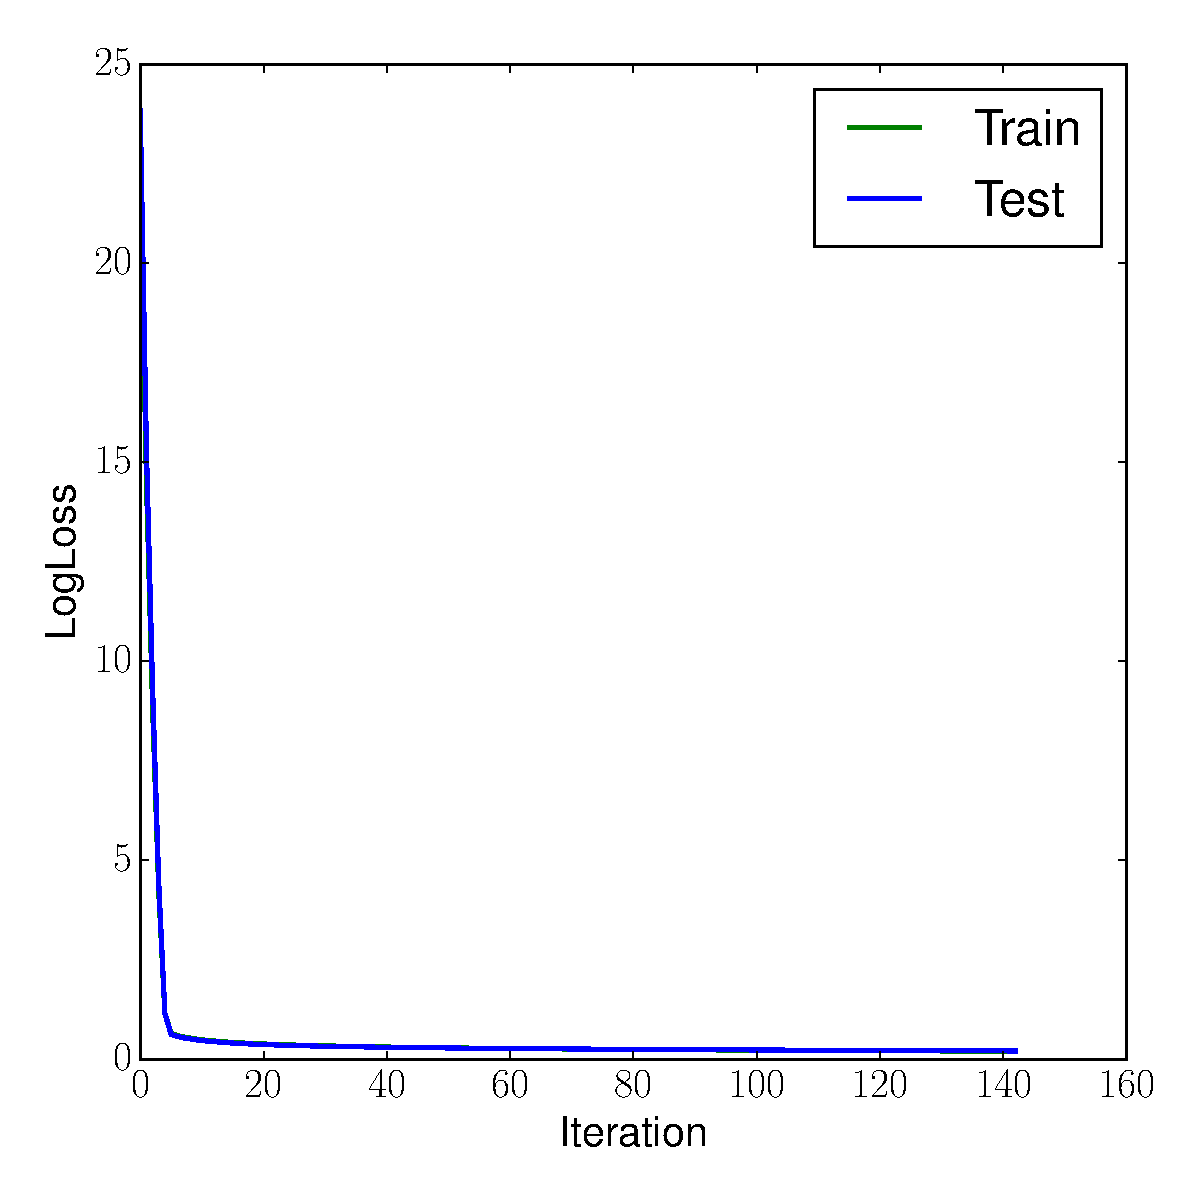
\includegraphics[width=\columnwidth]{mnist_bin_train_test_ll.pdf}
    \caption{Log loss as a function of iteration for both the MNIST training and testing datasets.  The log loss on the testing set was evaluated using the model parameters computed by fitting on the training set for each iteration.  Note how the loss decreases for both sets with each iteration as the fit improves.  In general, the testing loss is slightly larger than the training loss as expected.}
    \label{fig:mnist_bin_ll}
\end{figure}
\begin{figure}[H]
	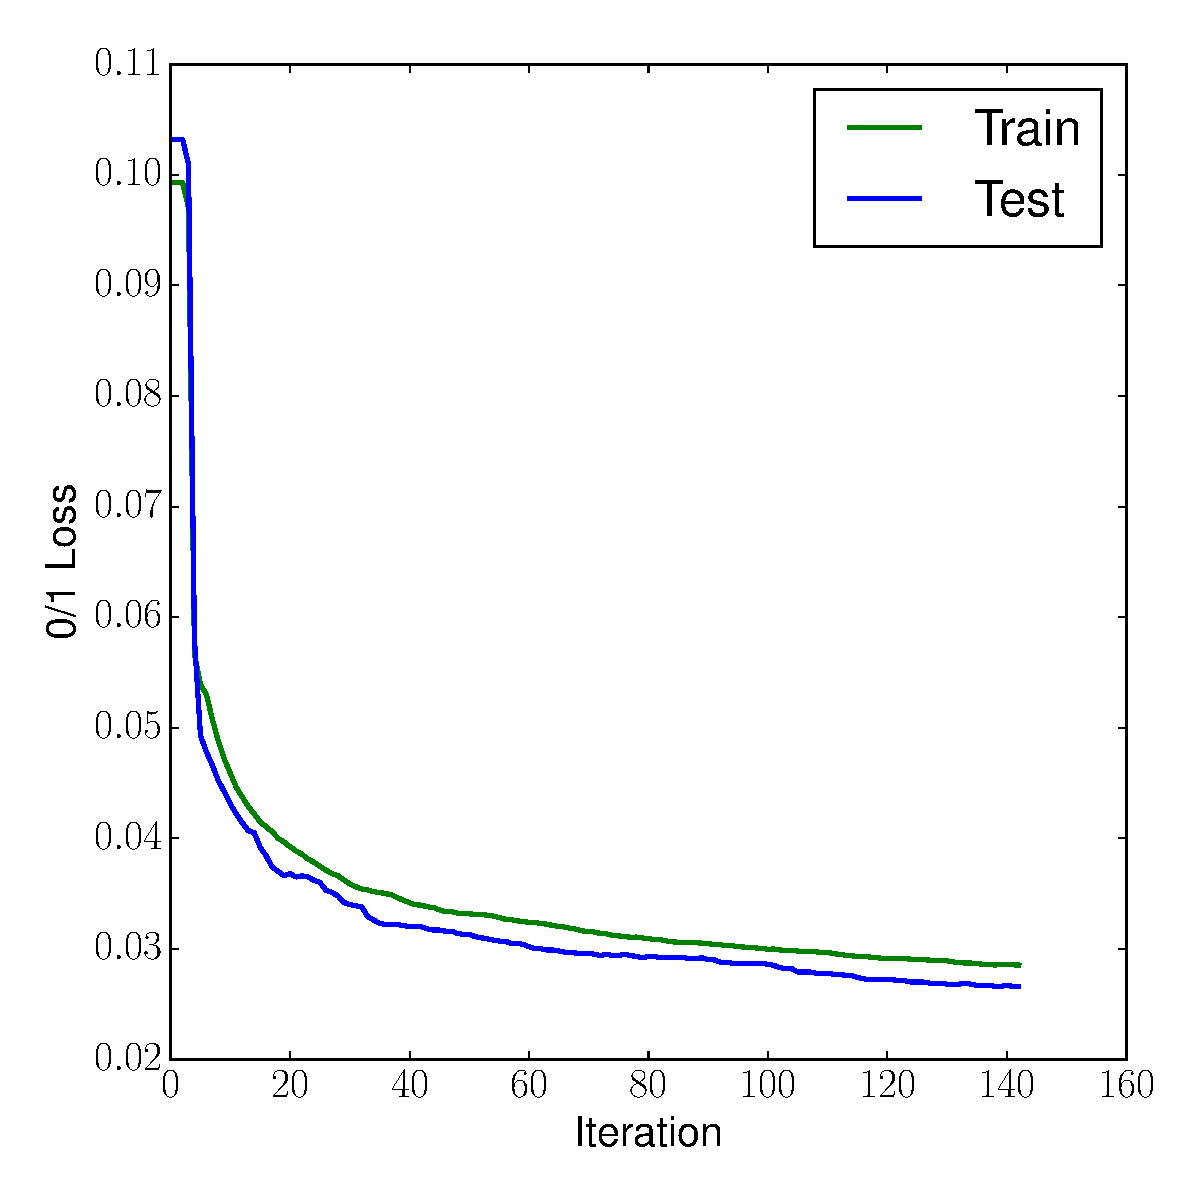
\includegraphics[width=\columnwidth]{mnist_bin_train_test_01.pdf}
    \caption{Caption Here}
    \label{fig:mnist_bin_01}
\end{figure}

\subsubsection*{2.1.3}
Given how the sigmoid binary logistic regression link function maps a prediction to a probability-like range $[0,1]$, a natural threshold for classification is to say if $\hat{y} > 0.5$, then $Y = 1$ and 0 otherwise as was assumed in lecture.  With this threshold, I found a training log loss and 0/1 loss of 0.54 and 0.051, respectively.  I found a testing log loss and 0/1 loss of 0.54 and 0.046, respectively.  Note that I normalized both losses by the size of each respective set for comparison's sake.

Note: On this question, I collaborated with Matt Wilde, Serena Liu, and Janet Matsen.

\end{document}